\subsubsection{Encrypt and decrypt}
\label{sec:sphinx:payload}

In contrast to the header, the integrity of the payload is not directly protected by the protocol. To ensure potential manipulations of the message remain visible to the final recipient, the content of the payload is hidden using a pseudorandom permutation scheme (PRP) and its inverse is used to undo the transformation. This comes with the property that if there were any modifications to the payload, such as a bit flip, the probability that the decoded message contains any relevant information is expected to be negligible.

To implement the PRP, HOPR uses the LIONESS \cite{lionesspaper} wide-block cipher scheme, instantiated by using Chacha20 as a stream cipher and BLAKE2s as a hash function as suggested by \href{https://katzenpost.mixnetworks.org/docs/specs/lioness.html}{Katzenpost}. See appendix \ref{appendix:lioness} for a detailed description and the chosen parameters.

As seen in Section \ref{sec:sphinx:keyderivation}, while creating the packet the sender derives a shared key $s_i$ with each node along the chosen path and uses them to create subkeys $s_i^{prp}$ to key the PRP. See Appendix \ref{appendix:keyderivation} for more details about the key derivation.

To allow the final recipient to determine whether a message is meaningful content or not, each message is padded by a protocol-specific tag $\tau$ and 0s to fit the packet size of 500 bytes, yielding $m_{pad}$. Decoded payloads that do not include $\tau$ are considered invalid and should be dropped.

\begin{figure}[H]
    \centering
    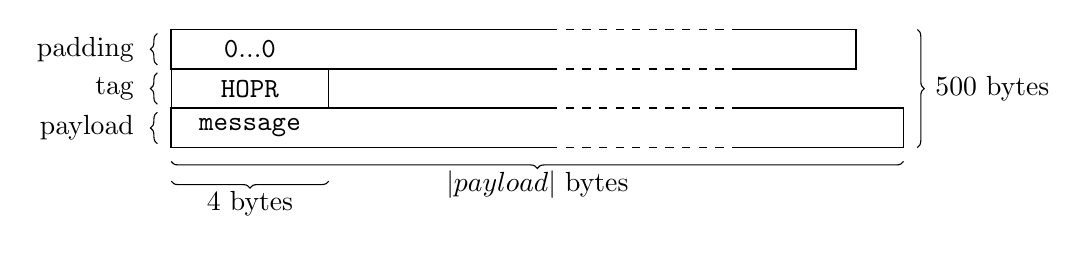
\begin{tikzpicture}
        \def\one{0.3}
        \def\lw{0.2}
        \def\middle{16*\one}
        \def\offset{8*\one}
        \def\packetLength{500}

        \def\paddingLength{29*\one}
        \def\payloadLength{31*\one}

        \foreach \i\text\message\width in{0/padding/$\mathtt{0...0}$/\paddingLength,1/tag/$\mathtt{HOPR}$/2,2/payload/$\mathtt{message}$/\payloadLength} {
                \begin{scope}[shift={(0,-\i*0.5)}]
                    \draw[decoration={brace,raise=5pt},decorate] (0,0.05) -- node[left=10pt] {\text} (0,0.5-0.05);
                    \path (0,0) -- (2,0.5) node[midway] {\message};

                    \ifnum\i=1
                        \draw [draw] (0,0) rectangle (2,0.5);
                        \draw (1,0.25) node {};
                    \else
                        \draw [line width=\lw mm] (\middle,0.5) -- (0,0.5) --  (0,0) -- (\middle,0);
                        \draw [line width=\lw mm] (\middle,0) --  (\middle+\offset, 0) [dashed];
                        \draw [line width=\lw mm] (\middle,0.5) --  (\middle+\offset, 0.5) [dashed];
                        \draw [line width=\lw mm] (\middle+\offset,0.5) -- (\width,0.5) --  (\width,0) -- (\middle+\offset,0);
                    \fi
                \end{scope}

            }

        \draw[decoration={brace,raise=5pt,mirror},decorate] (0,-1.0) -- node[below=5pt] {$|payload|$ bytes} (\payloadLength,-1.0);
        \draw[decoration={brace,raise=5pt,mirror},decorate] (0,-1.25) -- node[below=5pt] {4 bytes} (2,-1.25);

        \draw[decoration={brace,raise=5pt},decorate] (\payloadLength,0.5) -- node[right=8pt] {$\packetLength$ bytes} (\payloadLength,-1.0);
    \end{tikzpicture}
    \caption{Padded message consisting of 0-padding, protocol tag $\tau$ ($\mathtt{0x484f5052}$, ASCII-encoded ``HOPR"), and payload $m$.}
\end{figure}

The sender takes the padded message and encrypts it using $\mathsf{PRP.permutate}$ with the derived subkeys in reverse order ($...,s_{i+1}^{prp}, s_i^{prp}, s_{i-1}^{prp},....$)

$$\delta_i = \mathsf{PRP.permutate}_{s_i^{prp}}(\delta_{i+1})$$

where $\delta_4 = m_{pad}$ and $\delta_0$ is the ciphertext that is sent to the first relayer when using three intermediate hops.

Each node $n_i$ along the chosen path then removes one layer of encryption by setting

$$\delta_{i-1} = \mathsf{PRP.inverse}_{s_i^{prp}}(\delta_i)$$

yielding $\delta_0 = m_{pad}$ in case the node is the final recipient.

